
% this file is called up by thesis.tex
% content in this file will be fed into the main document

%: ----------------------- introduction file header -----------------------
\chapter{Conclusions and Future Work}

% the code below specifies where the figures are stored
\ifpdf
    \graphicspath{{11_future_work_and_conclusions/figures/PNG/}{11_future_work_and_conclusions/figures/PDF/}{11_future_work_and_conclusions/figures/}}
\else
    \graphicspath{{11_future_work_and_conclusions/figures/EPS/}{11_future_work_and_conclusions/figures/}}
\fi

% ----------------------------------------------------------------------
%: ------------------------------- content ----------------------------- 
% ----------------------------------------------------------------------

\section{Conclusions}

In this thesis, we have tackled the challenge of event summarization
from a~multimedia angle by leveraging social networks.
In the first part of the thesis,
we have presented the Semantic Web,
its technologies, and its applications like Linked Data.
In continuation, we have discussed social networks
and their features and have classified them
based on their level of media item support.
We have applied semantic methods for limiting ambiguity
that is intrinsic to language and that especially affects
short textual microposts, which oftentimes lack context.
As this task required the orchestration of several services
in combination, we have shown how provenance information
can be preserved to make the involved steps traceable.
We have shown how Wikipedia edits
that we capture in realtime can be clustered by language
for the task of detecting breaking news event candidates.
An accompanying application called \emph{Wikipedia Live Monitor}
was developed and publicly released in the same context.
We have examined how media items can be extracted from 
various social networks and how the different
underlying social network messages and interactions
can be aligned by an abstraction layer.
Further, we have introduced an algorithm
to detect camera shots in streaming video and 
annotated them semantically with media fragments URIs.
This task is a~required step for video deduplication,
which we have tackled together with photo deduplication.
We have determined social-network-specific reasons
for the occurrence of duplicate and near-duplicate content
on social networks.
Based on these findings, we have developed and algorithm
that is tailored to detect such occurrences of duplicate
and near-duplicate content.
This algorithm has multiple matching conditions,
which makes it hard for a~non-expert user to determine
why or why not media items have been matched.
Driven by this observation, we have researched
if speech synthesis together with dynamic media fragment creation
can help non-expert users understand the algorithm's output,
which in consequence allowed us to significantly improve it.
We have introduced a~ranking formula for social media clusters
that, based on a~social interaction abstraction layer,
ranks clusters by popularity and from each cluster selects
the visually most appealing cluster representative media item.
Afterwards, we have discussed and evaluated several
media gallery compilation algorithms
that fulfill media gallery aesthetics criteria,
which we have defined.
Finally, we have created an interactive,
speech-synthesis-supported visualization format
on top of our media gallery compilation algorithms.

Based on a~very open event definition from WordNet---%
\textit{``something that happens at a~given place and time''}---%
we have identified the need to
visually and audially summarize events
of personal or public interest.
The increasingly important role of first-hand eye-witness
social media data at recent events like the
Boston Marathon bombings 2013%
\footnote{\url{http://en.wikipedia.org/wiki/Boston_Marathon_bombings}, accessed July 15, 2013}
or the Occupy Gezi movement 2013 in Turkey%
\footnote{\url{http://en.wikipedia.org/wiki/2013_Taksim_Gezi_Park_protests}, accessed July 15, 2013}
drastically confirm the observation that there is a~strong demand
for social-network-based event summarization.
Since the beginning, we have openly shared our progress
in form of screenshots for the different tasks
of the application
(\url{http://twitpic.com/tag/TomsPhD}, accessed July 15, 2013)
and have also documented our progress in general
(\url{http://tomayac.com/tweets/search?q=%23TomsPhD}, accessed July 15, 2013).
This has allowed us to get early feedback on ideas
and visualizations already at the design phase.
The way interactive mode works in media galleries
that was detailed in \autoref{sec:interactivemediagalleries}
is a~result of this early-stage feedback loop. 
An earlier iteration of interactive mode
is documented in the screenshot available at
\url{http://twitpic.com/c94j02} (accessed July 15, 2013),
where the background media items were already blurred,
but not yet transformed into black-and-white.
Especially with media items of type photo,
through steadily monitoring (at time of writing) current events,
we have learned that social media galleries
need to be specifically tailored to handle all sorts of photo formats,
as screenshots in non-standard aspect ratios
are more common than expected.
Some examples are documented in a~screenshot available
at \url{http://twitpic.com/bvjmgc} (accessed July 15, 2013).
We were also surprised by the diversity of the media items
related to a~given event.
Where media galleries of traditional sources
like news agencies feature strictly event-related media items,
media galleries created by our approach also feature
media items of humorous nature like memes,%
\footnote{An Internet meme is an idea, style, or action that spreads, often as mimicry, from person to person via the Internet, as with imitating the concept}
photo montages,
or parody images.
On the one hand, this can be attributed to the less formal requirements
regarding the political correctness of media galleries 
created through our approach.
On the other hand, it can be traced back to the insouciant naivety
of non-professional photographers and cinematographers
that are responsible for the majority of social network media items on the other.
A~good example is documented in the screenshot available at
\url{http://twitpic.com/bvwz7x} (accessed July 15, 2013).

Our initial research question was the following.
\textit{``Can user-customizable media galleries
that summarize given events be
created solely based on textual and multimedia data
from social networks?''}
Concluding, the answer is clearly \emph{yes}.
Media galleries based on social network multimedia data 
are faster to generate, more authentic and concise,
more flexible and customizable, more comprehensive and diverse, and finally oftentimes more interesting to consume than
traditional media galleries.
For any serious use case, human final inspection will
always be required, even in the long-term,
as we will outline in the next subsection.
With our research and the applications
\emph{Social Media Illustrator} and \emph{Wikipedia Live Monitor},
we have contributed valuable tools,
methods, design ideas, and algorithms
to facilitate and automate the otherwise tedious task
of manually generating media galleries.
This allows users of these applications
to focus on tasks where humans excel,
like, \emph{e.g.}, interpreting the effect of events on society,
putting events in relation to each other,
or identifying reasons that caused them.

\section{Future Work}

\subsection{Media Item Verification}

An aspect that we have left aside so far is the \emph{verification}
of the \emph{credibility} and \emph{authenticity} of both sources
and media items themselves that get shared on social networks.
The growing importance and usage of truly first-hand eyewitness
social media in traditional news media---%
or even social media being \emph{the} actual news,
as to some extent it was the case with the Boston Marathon bombings,
makes social networks also an increasingly popular focus of \emph{intentionally false information}.
The distribution of false information in form of media items
can have all sorts of motivations, ranging from (sometimes fun)
hoaxes\footnote{A hoax is a~deliberately fabricated falsehood made to masquerade as truth}
to political propaganda to simple human errors.
The list is far from being complete.
Occurrences of false information can include
media items stemming from unrelated events being published as event-related,
manipulation  of photos or videos to modify, add, or remove persons or objects in media items,
or wrong statements in the accompanying microposts.
Manual approaches to recognize false information 
can include carefully checking the account publishing history
of the originating source (does the social network user seem legit?),
comparison of depicted scenes with independent media,
\emph{e.g.}, satellite imagery or street panoramas
(does the depicted scene look the same elsewhere?),
verifying weather conditions
(were the known weather conditions at the time
when the event happened the same as the depicted ones?),
analyzing media items for known patterns of pixel manipulation
(are traces of, for example, image editing software usage visible?),
or finally, verifying media item metadata
(do the data in the Exif block look valid?).
Research on media item verification is ongoing,
an example is~\cite{gupta2013fakingsandy} by Gupta \emph{et~al.}
The first commercial companies are beginning to offer media item 
verification as a~service, \emph{e.g.}, Storyful (\url{http://storyful.com/}).
The Managing Editor of the company, Markham Nolan,
has covered the topic of media item verification
in a~TED Talk, which is available online.%
\footnote{\url{http://www.ted.com/talks/markham_nolan_how_to_separate_fact_and_fiction_online.html},
accessed July 15, 2013}
A~future research direction can be to automate
this entirely manual process, albeit, having a~human in the loop
will---all potential automation aside---still be required
and desirable for many use cases.

\subsection{Evaluation of Subjective Data}

\paragraph{Examples of Subjective Data:}

In many of the tasks from the previous chapters
we had to deal with subjective data and how to evaluate it.
In contrast to \emph{objectivity} (where people see things
from a~standpoint \emph{free} from human perception and its influences,
human cultural interventions, past experiences,
and expectation of the result),
the contrasting term \emph{subjectivity} is used to refer to the condition
of being a~\emph{subject}, under the influence of the subject's perspective, experiences,
feelings, beliefs, and desires~\cite{honderich2005oxford}.
In the following, we list some of the subjective things
that were evaluated in this thesis.
As a~first example, there are media gallery aesthetics and media gallery usefulness
(\autoref{cha:media-item-compilation}),
where the subjective decision is whether
or not generated media galleries are aesthetically pleasing 
and at the same time useful for getting an understanding
of the summarized event.
Further examples are the subjective decisions on a~media item set's
ranking (\autoref{cha:media-item-ranking}),
its clustering and deduplication (\autoref{cha:media-item-deduplication}, \autoref{cha:shot-boundary-detection}),
and the set itself (\autoref{cha:media-item-extraction}).
In addition to that, there is also event detection,
where the subjective decision is whether or not a~given detected breaking news event candidate is indeed newsworthy (\autoref{cha:eventdetection}) and for whom.
Finally, there are the extracted and disambiguated named entities
from the accompanying microposts for media items
(\autoref{cha:micropost-annotation}).

\paragraph{Subjective Data Evaluation Strategies:}

Common strategies for the evaluation of subjective data were 
examined by Brabb and Morrison in~\cite{brabb1964evaluation}.
In the multimedia context, the main evaluation strategies are
the use of Likert scales~\cite{likert1932likertscale} 
and the Mean Opinion Score~\cite{itu1998mos},
which we have chosen for our evaluation purposes,
as we were mainly interested in the perceived quality of our tasks.
What all these evaluation strategies have in common is
that they create a~potentially artificial test feeling
or lab environment situation, where users tend to not act naturally.

\paragraph{Multi-Armed Bandits Experiments:}

One-armed bandits are slot machines
with potentially varying expected payout.
Multi-armed bandit experiments are hypothetical experiments
where, when faced with several one-armed bandits,
the objective is to determine the most profitable one.
The compromise or tension with such experiments is to
greedily decide on bandits that have performed well in the past
and taking the risk of trying new ones.
Highly developed mathematical models exist~\cite{scott2010bandits}
to optimize this problem.
Compared to more classical A/B tests, where two variants 
are tested against each other, multi-armed bandit experiments
are statistically just as valid and can oftentimes return results earlier, as already during the experiment
more focus is gradually put on well-performing variants.

In the online retail industry, multi-armed bandit experiments
have found broad adoption as they are easy to set up and efficient in finding actionable results.
They are used extensively, \emph{e.g.}, for the optimization 
of conversions for things like
online purchases, newsletter sign-ups, or click-throughs.
Typical experiment factors are heading texts, button colors and shapes,
as well as page layout variants.
Multi-armed bandits experiments are in consequence standard features
of common off-the-shelf Web analytics software like, for example,
Google Analytics (\url{http://google.com/analytics}).

Our hypothesis is that multi-armed bandit experiments can be used 
to evaluate the sort of subjective data we generate
with our application \emph{Social Media Illustrator}, given that we 
properly define our optimization criteria.
Unlike with, \emph{e.g.}, online purchases,
where the optimization criterion are conversions,%
\footnote{The amount of people who do not just put items in the virtual shopping cart,
but who then proceed to and successfully complete the checkout process}
with media galleries there is no direct optimization criterion.
However, our assumption is that we can use indirect criteria like
interaction with the media gallery
as outlined in \autoref{sec:interactivemediagalleries},
the rationale being that if
a~media gallery is interesting, the user will interact with it.
Common Web analytics software is capable of tracking mouse and
keyboard events that occur when users interact with Web pages.
By exploiting this fact, we can attach event listeners
to media galleries and report these events
to the Web analytics software running on a~remote server.
By varying media gallery styles and parameters like the width,
number of contained items, item size, \emph{etc.},
we can then over time determine promising candidates.
The proposed evaluation approach is less expensive
and more scalable than user studies,
albeit user studies may still outperform the approach
with regard to discovering aspects that were not part
of a~multi-armed bandit experiment and thus never tested,
but that a~study participant may have noted in a~free-form question.
In the long-term, the proposed approach
can thus be the seed for \emph{more targeted user studies}.

\subsection{Application Domains}

\paragraph{Embedded Media Galleries:}

A final future research direction is finding new application domains.
With our examples so far, we have mainly focused
on the (online) journalist use case.
We envision interactive media galleries taking the place
of static photo galleries (\autoref{fig:occupygezibbc})
or embedded videos on online editions
of news websites or Web portals.

\paragraph{Data Journalism:}

Data journalism~\cite{rogers2011datajournalism,gray2012data}
is a~form of journalism that reflects the increased role
of numerical data in the production and distribution of information
in the digital era.
It touches on the fields of design, computer science, and statistics.
Interactive media galleries and the cross-network search capabilities enabled by our application \emph{Social Media Illustrator}
can greatly facilitate the data journalism task of researching news stories and exploring multimedia data.

\paragraph{Event Pages of Social Networks:}

Some social networks like Facebook or \googleplus
offer their users the creation of events where
event-related media items can be manually or automatically
uploaded when event attendees \emph{check in} to an event.
Naturally, interactive media galleries embedded on
social network sites themselves will only feature media items
from the social network in question and not include foreign ones.

\paragraph{Disaster Response:}

Disasters like earthquakes, floods, plane crashes, \emph{etc.}\ cause
great damage or even loss of lives.
Disaster response includes measures to
mitigate the effects of a~disastrous event
in order to avoid further loss of lives or property.
Social networks and especially social media
play an increasing role in disaster response%
~\cite{shklovski2008disasterresponse,sutton2008backchannels}.
Our work has already sparked initial interest~\cite{meier2013wikipedia}
in the disaster response community.
We will focus future work primarily on this aspect.

\subsection{Commercial Activity in the Field of Social-Network-Based Event Summarization}

The research fields of event summarization and event archiving
based on social network multimedia data have resulted in 
interesting business creations in recent months.
Albeit similarities to our work exist,
there are still many differences in the details.

\paragraph{Mahaya:}
 
The company Mahaya has launched a~beta-version
of a~commercial automatic event archiving tool called Seen
(\url{http://beta.seen.co/}),
which, based on manually entered event metadata like event name,
location, and dates, uses a~necessarily provided Twitter hashtag
to create a~complete and permanent archive of all event-related tweets,
media items, and slide decks.
Based on term frequency and co-occurrence analyses,
the event is split into subevents
and each subevent's hot topics are tried to be detected.
The application's main data source is Twitter,
links to certain media hosting platforms are followed.
At time of writing, Seen does not yet deduplicate and cluster
similar media items,
albeit the tool is being actively worked on.
A~screenshot of Seen can be found in \autoref{fig:seen}.

\begin{figure}
  \centering
  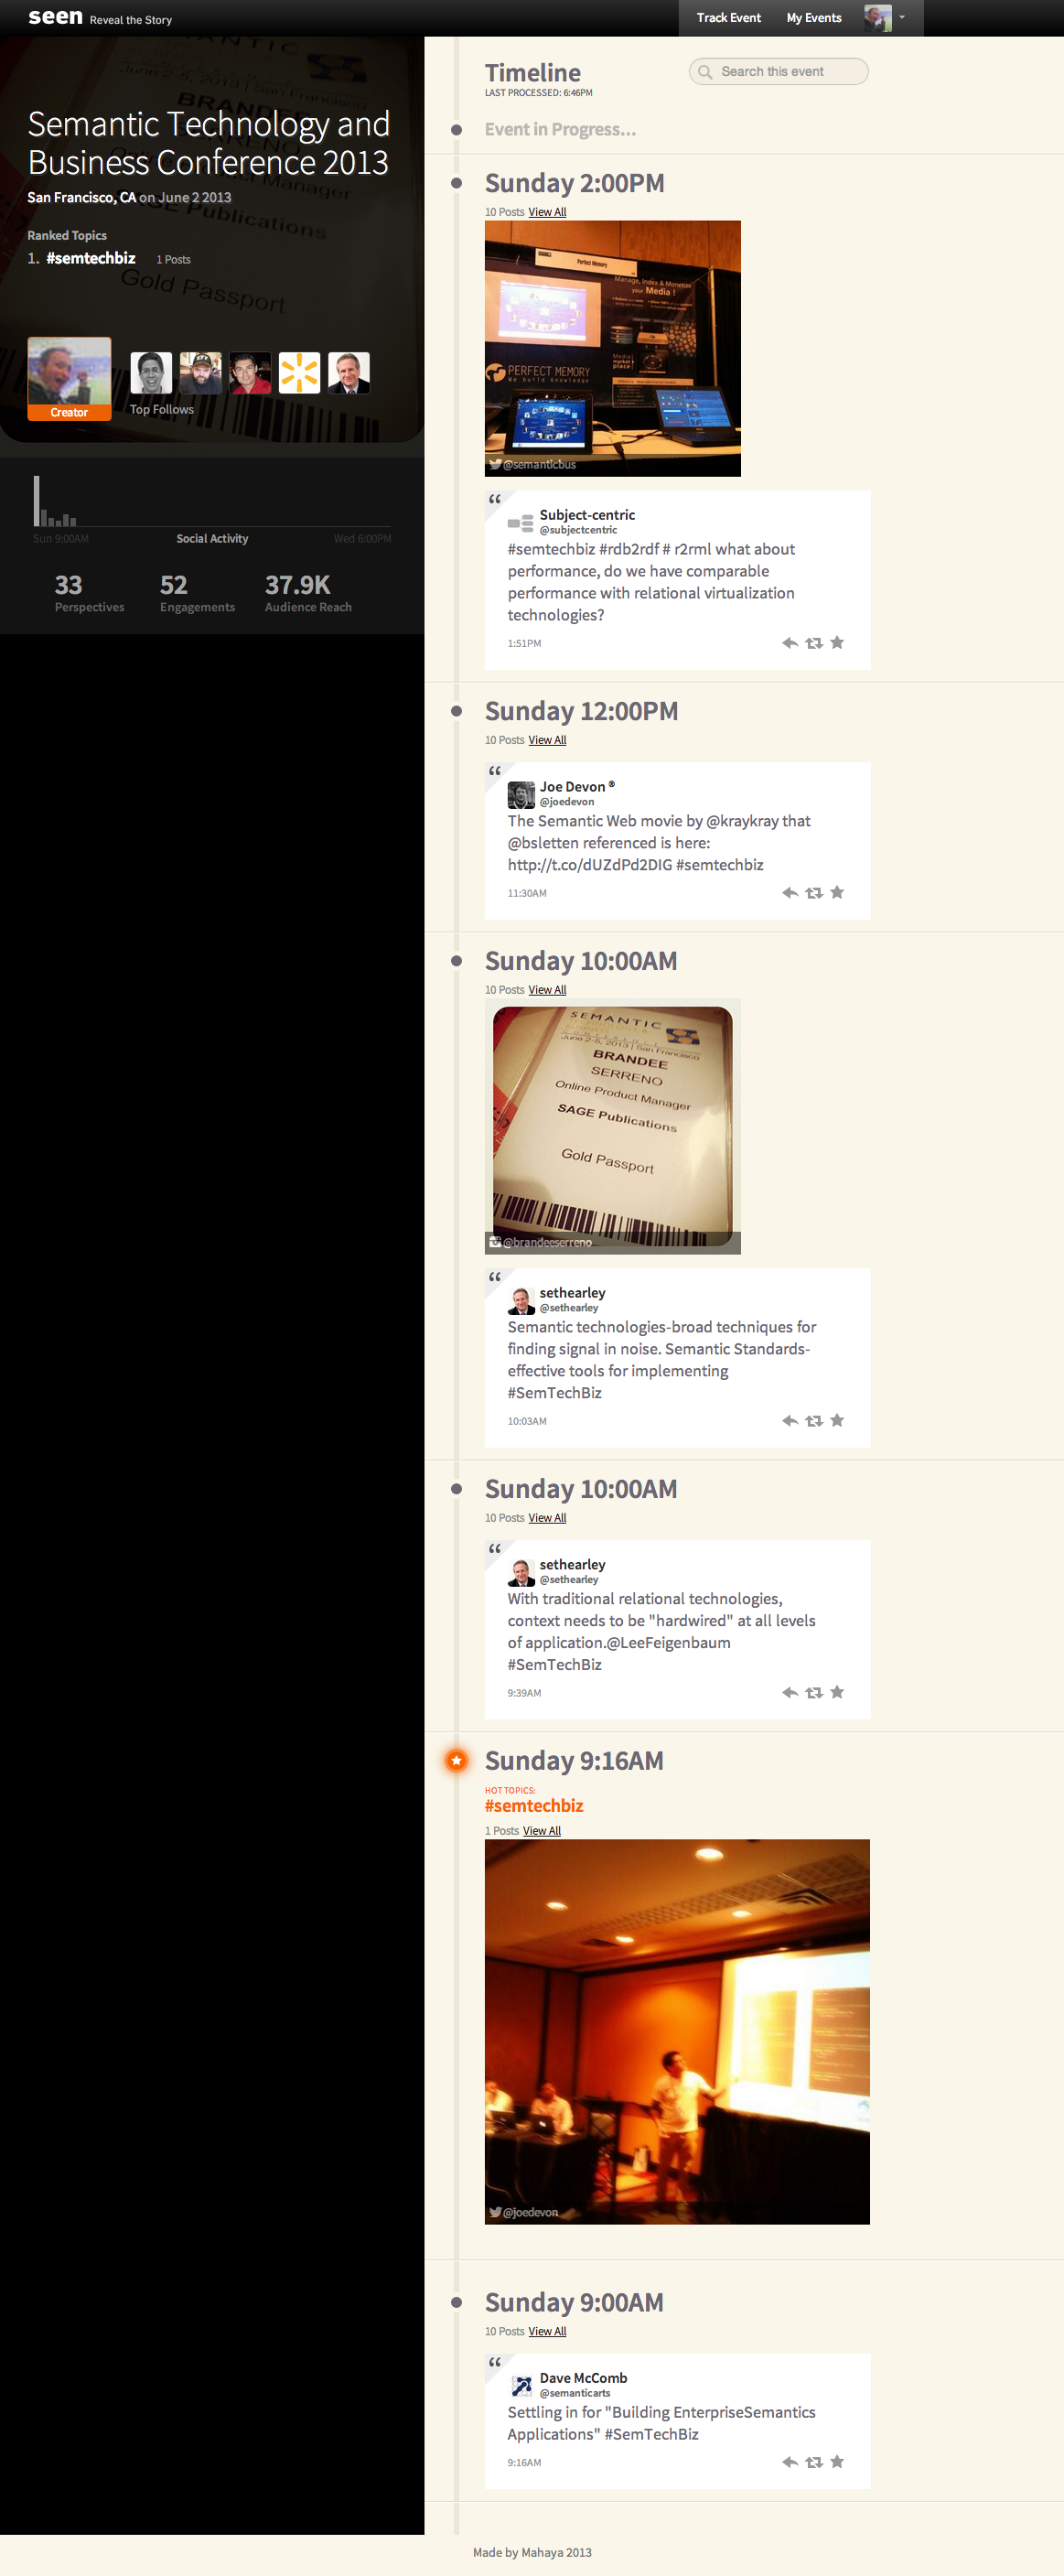
\includegraphics[width=0.95\textwidth,height=0.9\textheight,keepaspectratio]{seen.png}
  \caption[Mahaya's commercial automatic event archiving tool Seen]{Mahaya's commercial automatic event archiving tool Seen
    (\url{http://beta.seen.co/})}
  \label{fig:seen}
\end{figure}

\paragraph{Eventifier:}

Eventifier \url{http://eventifier.co/}) is a~commercial tool
that facilitates the automated permanent archiving of events
in form of event-related photos, videos, tweets, slide decks, 
and event contributors.
Similar to Mahaya's product Seen,
the application's main data source is Twitter.
The manually entered official event hashtag and potentially existing
official Twitter account serve to encounter event-related content.
At time of writing, Eventifier does not yet
deduplicate and cluster similar media items,
however, this feature is said to be implemented.
A~screenshot of Eventifier can be seen in \autoref{fig:eventifier}.

\begin{figure}
  \centering
  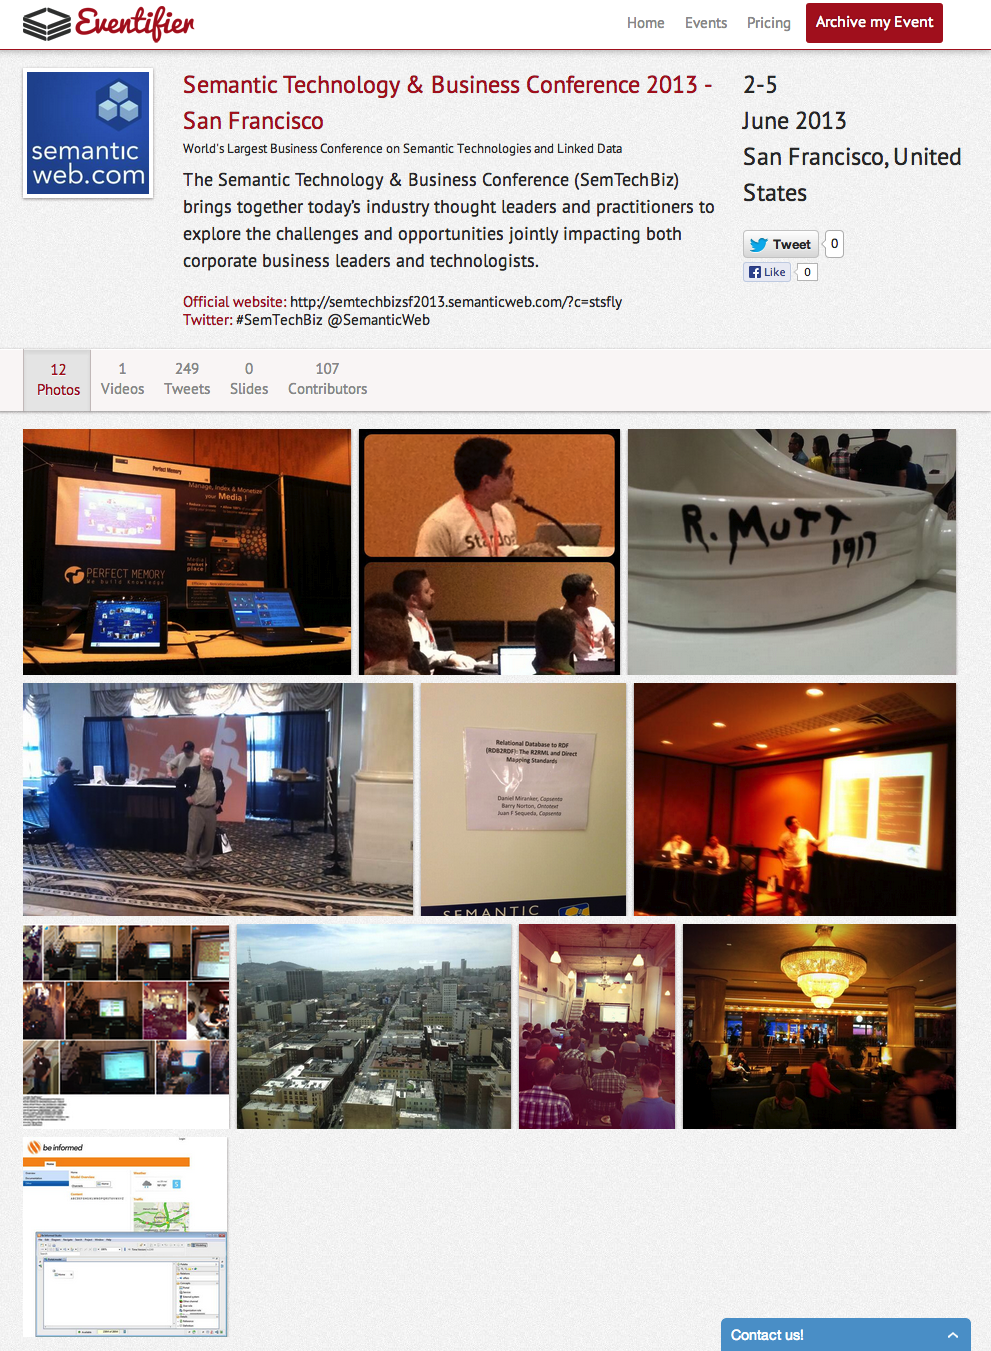
\includegraphics[width=0.95\textwidth,height=0.9\textheight,keepaspectratio]{eventifier.png}
  \caption[Automated commercial event archiving tool Eventifier]{Automated commercial event archiving tool Eventifier
    (\url{http://eventifier.co/})}
  \label{fig:eventifier}
\end{figure}

\paragraph{Storify:}

The commercial tool Storify (\url{http://storify.com/})
allows for the manual compilation of
event-related media items, articles, and microposts
to generated permanently available stories
that---depending on the level of human curation---%
can efficiently summarize an event.
Storify does not deduplicate and cluster
similar media items.
A~screenshot of Storify can be seen in \autoref{fig:storify}.

\begin{figure}
  \centering
  \includegraphics[width=0.95\textwidth,height=0.9\textheight,keepaspectratio]{storify.png}
  \caption[Manually assisted commercial event archiving tool Storify]{Manually assisted commercial event archiving tool Storify
    (\url{http://storify.com/})}
  \label{fig:storify}
\end{figure}

\paragraph{Media Finder:}

Media Finder (\url{http://mediafinder.eurecom.fr/})
is an academic non-commercial tool that
has advanced named entity centric clustering capabilities
based on extracted named entities in microposts.
Media items can be clustered by topic, named entity,
named entity type, and micropost instance.
We have contributed the application's media extraction component,
in consequence the covered social networks
are exactly as described in \autoref{cha:media-item-extraction}.
A~screenshot of Media Finder can be seen in \autoref{fig:mediafinder}.

\begin{figure}
  \centering
  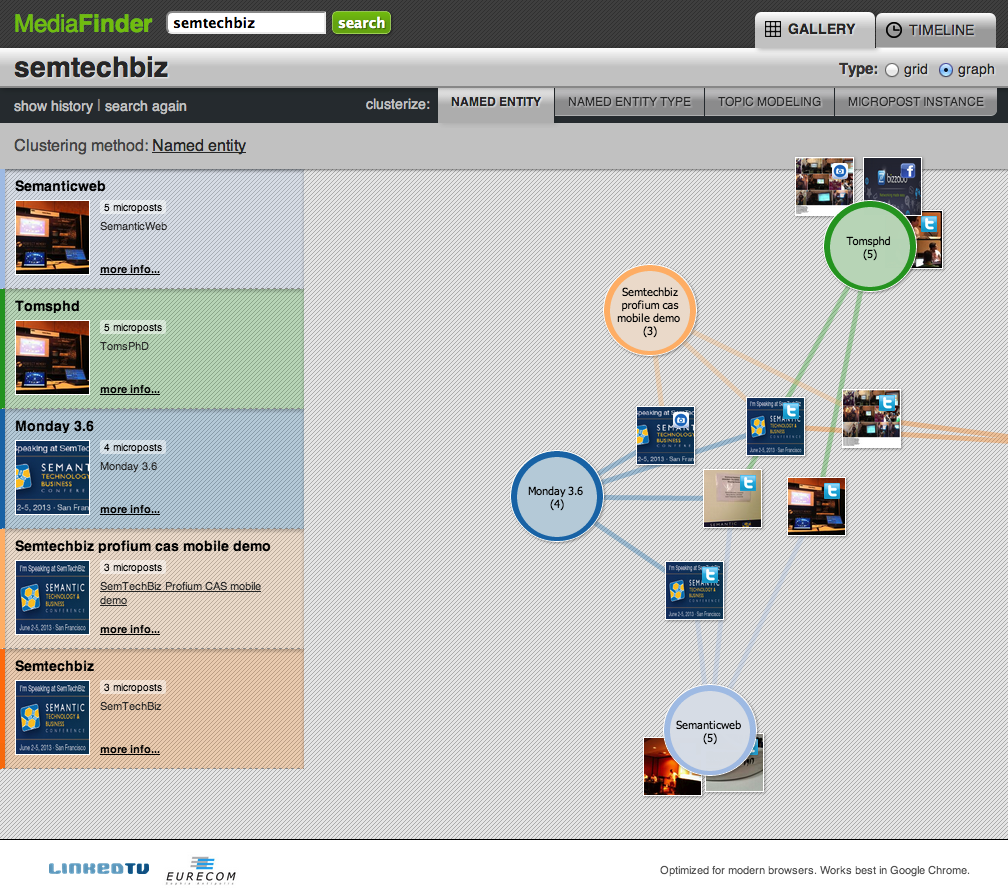
\includegraphics[width=0.95\textwidth,height=0.9\textheight,keepaspectratio]{mediafinder.png}
  \caption[Academic event summarization tool Media Finder]{Academic event summarization tool Media Finder (\url{http://mediafinder.eurecom.fr/})}
  \label{fig:mediafinder}
\end{figure}

\subsection{Comparison of Tools}

In the previous paragraphs, we have characterized
commercial and non-commercial tools for the tasks
of event summarization and event archiving. 
\autoref{table:toolcomparison} shows how these tools
compare against our own application \emph{Social Media Illustrator},
which, for reference, is depicted again in \autoref{fig:socialmediaillustrator}.
What sets our application apart
are its interactive media galleries that,
together with speech synthesis as outlined in \autoref{sec:interactivemediagalleries}
allow for novel kinds of experiences when it comes to 
event summary consumption.

\begin{figure}
  \centering
  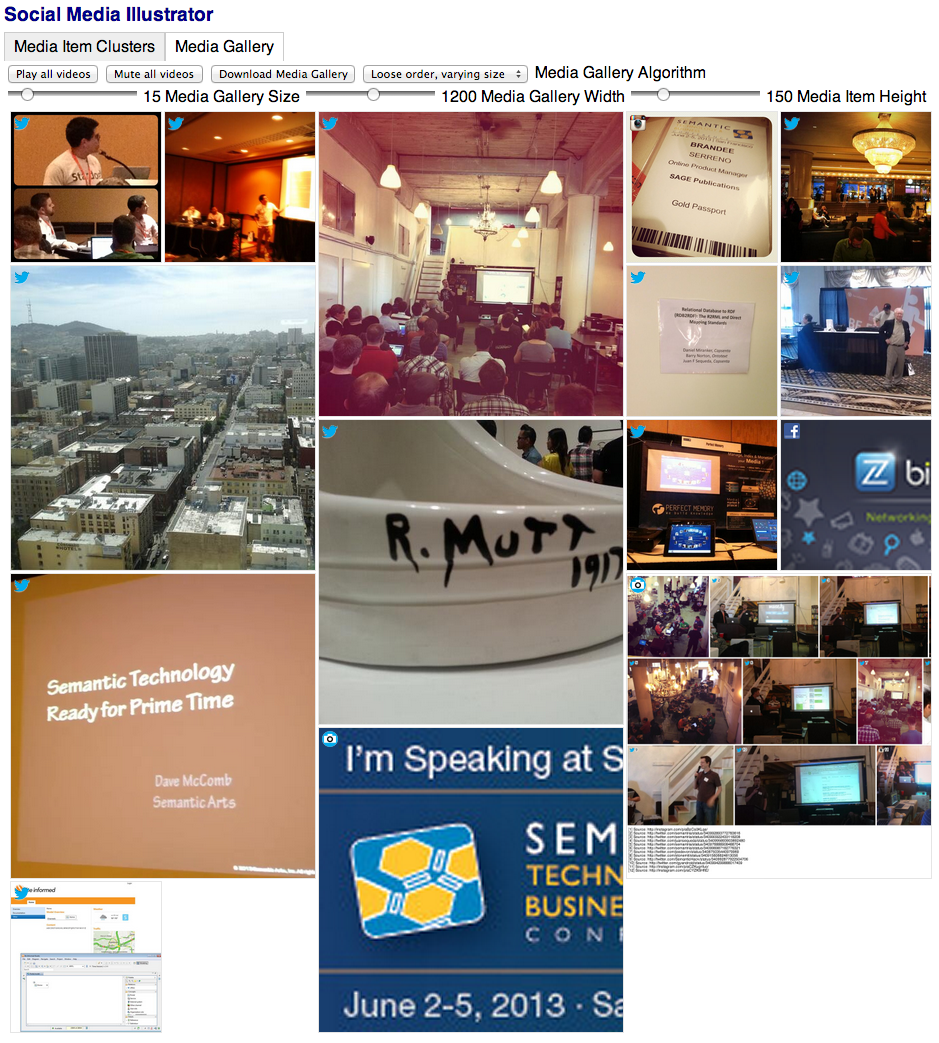
\includegraphics[width=0.95\textwidth,height=0.9\textheight,keepaspectratio]{socialmediaillustrator.png}
  \caption[Our own academic event summarization tool \emph{Social Media Illustrator}]{Our own academic event summarization tool \emph{Social Media Illustrator} (\url{http://social-media-illustrator.herokuapp.com/})}
  \label{fig:socialmediaillustrator}
\end{figure}

\begin{sidewaystable}[!ht]
  \centering
  \small
  \begin{tabular}{|l|l|l|l|l|l|}
    \hline
    \textbf{Tool} & \textbf{Seen} & \textbf{Eventifier} & \textbf{Storify} & \textbf{Media Finder} & \textbf{Social Media Illustrator}\\ \hline
      \hline
      \textbf{Data source} & Twitter & Twitter & Multiple & Multiple & Multiple\\
      \textbf{Main task} & Archiving & Archiving & Summarization & Summarization & Summarization\\
      \textbf{Operation mode} & Automated & Automated & Manual & Semi-automated & Semi-automated\\
      \textbf{Linkable} & Yes & Yes & Yes & Yes & No\\
      \textbf{Downloadable} & No & No & No & No & Yes\\
      \textbf{Customizable} & No & No & Yes & Yes & Yes\\
      \textbf{Interactive} & No & No & No & No & Yes\\
      \textbf{Commercial} & Yes & Yes & Yes & No & No\\
      \hline
    \end{tabular}
    \caption[Comparison of event archiving and summarization tools]{Comparison of commercial and non-commercial event archiving and summarization tools \todo{Check final orientation}}
  \label{table:toolcomparison}
\end{sidewaystable}

\section{Closing Words}

In this thesis, we have touched on multiple areas of research.
Some of the encountered problems and challenges,
for example, named entity extraction and disambiguation
for short and oftentimes sloppily-authored microposts
or also video deduplication,
certainly deserve a~thesis of their own.
We have opted for a~pragmatic approach in such cases
and have not shied back from either using third-party tools
or working with approximations or heuristics, 
which work well enough for our use case.
From the beginning, we have envisioned an application
that would facilitate the tedious work
of compiling media galleries manually.
This application, \emph{Social Media Illustrator},
forms part of the deliverables of the thesis.
We have separated the task of building this application
in several actionable steps and have contributed 
scientific publications for each of them.
The chapters of this thesis follow these steps loosely.  
As a~reminder, the concrete steps were the following:
(i)~micropost annotation,
(ii)~event detection,
(iii)~media item extraction,
(iv)~media item deduplication,
(v)~media item ranking, and
(vi)~media item compilation.
At the end of this thesis,
we are now in the position to first accurately detect events
and second, to visually and audially summarize them
in an optionally fully-automated or semi-automated manner,
so the circle has been closed.

We were ourselves surprised by the broad range
of possible future use cases, ranging from end users
reviving the atmosphere of a~concert,
to data journalists researching political events
of potentially global interest,
to finally disaster relief workers coordinating 
their efforts based on information derived from our applications.
We are excited to improve, extend, and adapt
\emph{Social Media Illustrator} and \emph{Wikipedia Live Monitor}
in the future with concrete future research opportunities
that were outlined earlier in this chapter.
This thesis marks the end of this doctorate,
but it certainly does not mark the end of this work.

\begin{flushright}
\textit{``The Software shall be used for Good, not Evil''}.%
\footnote{\url{https://github.com/douglascrockford/JSLint/blob/master/jslint.js\#L16},
accessed July 15, 2013}~---Douglas Crockford
\end{flushright}

\section*{Chapter Notes}
This chapter is partly based on the following publications:
\todo{Add publications}

\bibliographystyle{plainnat}
\bibliography{backmatter/references}